%%%%%%%%%%%%%%%%%%%%% chapter.tex %%%%%%%%%%%%%%%%%%%%%%%%%%%%%%%%%
%
% sample chapter
%
% Use this file as a template for your own input.
%
%%%%%%%%%%%%%%%%%%%%%%%% Springer-Verlag %%%%%%%%%%%%%%%%%%%%%%%%%%
%\motto{Use the template \emph{chapter.tex} to style the various elements of your chapter content.}
\chapter{Execution Time and Analysis}
\label{Introduction}
The interest of this study was to analyse the execution times of the three algorithms described above, to determine which method executes in the fastest time and thus might be most appropriate for using to solve large problems. The execution times were measured for each method for domains of the following sizes with a maximum frequency of 500Hz for FDTD and PSTD in 3D, and 1kHz for SFDTD in 2D:\\
\begin{center}
\begin{tabular}{|c|c|c|c|} 
  \hline
 Dimension ($m^2$) & FDTD Cells & SFDTDCells & PSTD Cells \\
 \hline
 5 & 121104	& 121104 & 24025\\ 
 10 & 483025 & 483025 & 62500\\  
 20 & 1932100 & 1932100 & 192721\\ 
 40 & 7722841 & 7722841 & 667489\\ 
 60 & 30880249 & 30880249 & 2474329\\ 
 \hline
\end{tabular}\\
\end{center}

The time step execution time was evaluated for 2000 executions, allowing for smaller or larger required time steps to be part of the analysis. The execution of each time step includes only the steps outlined above, with no plotting. Execution time was measured using Matlabs Tic and Toc functions. During execution, Matlab was the only task running in the foreground of the system, but background tasks were allowed to continue without restriction. The computer system used for these tests had the following properties:\\

\begin{itemize}
\item Intel Core i5 4690k CPU @ 4.5GHz @ 1.227V
\item 16GB DDR3 RAM @ 3875.3MHz
\item Asus Gryphon Motherboard with Z97 Chip Set
\end{itemize}



\section{Results}
The average execution time for each method is given below: \\
\begin{figure}[H]
\centering
  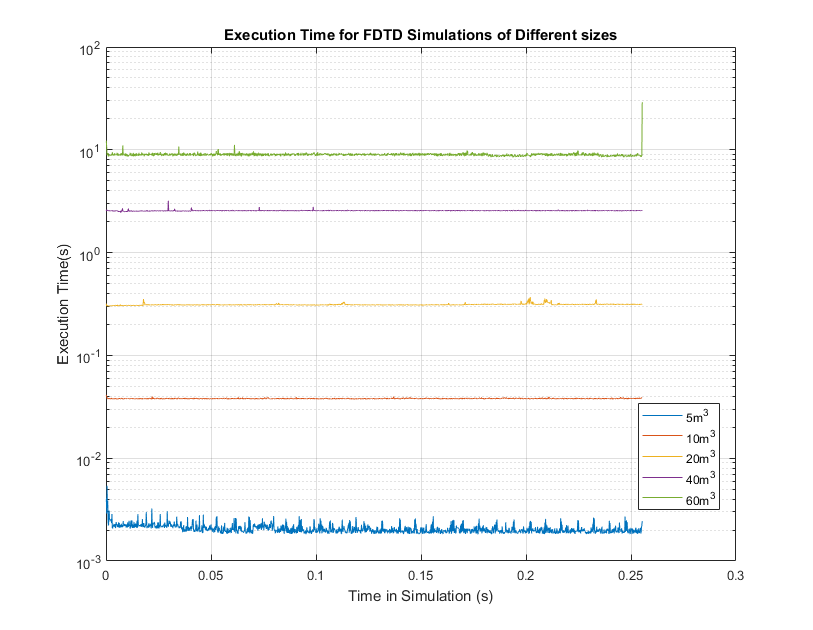
\includegraphics[width=\textwidth]{./graphics/FDTD simulation execution time.png}
  \caption{Execution times for FDTD simulations in domains of increasing size}
\end{figure}

\begin{figure}[H]
\centering
  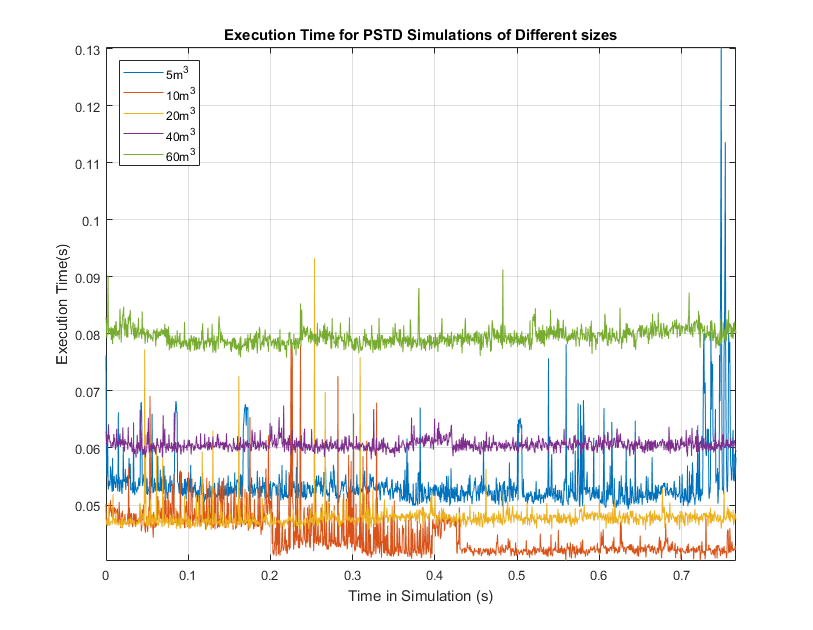
\includegraphics[width=\textwidth]{./graphics/PSTD Simulation Execution Times.png}
  \caption{Execution times for PSTD simulations in domains of increasing size}
\end{figure}

\begin{figure}[H]
\centering
  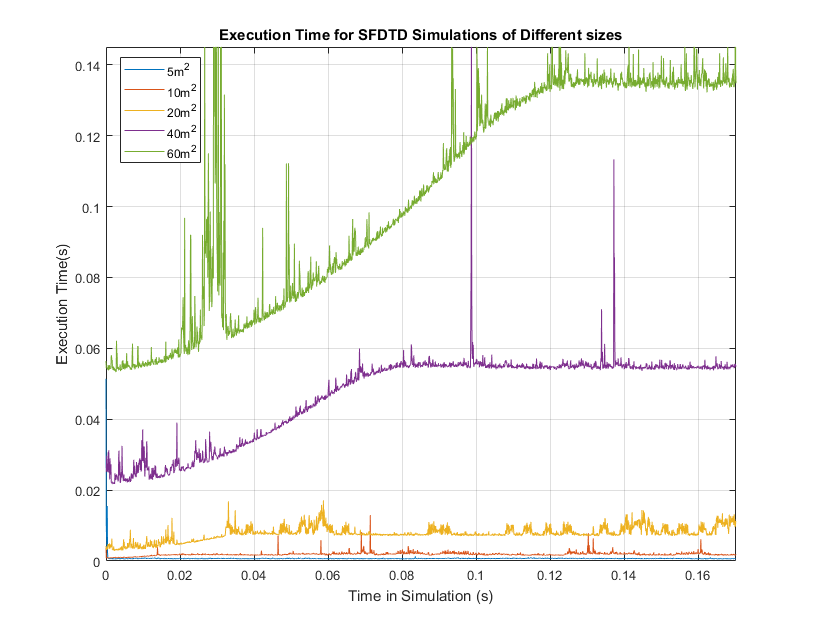
\includegraphics[width=\textwidth]{./graphics/SFDTD simulation execution time.png}
  \caption{Execution times for SFDTD simulations in domains of increasing size}
\end{figure}

\section{Analysis}
These results how some interesting properties of simulation execution over time for the different methods. The FDTD method is significantly slower at executing than the PSTD and SFDTD methods, particularly with the larger domains. The arrogate execution time for $0.25s $of simulation for a $40m^3$ domain was 1 hour 5 minutes. Where as execution for the same domain in PSTD was 1.5 minutes. Execution time data for the PSTD method appears to fluctuate wildly compared to the FDTD data, and this is probably due to the influence of system loading by background tasts. These fluctuations are better masked by the log scaling in time for the plot of FDTD execution time data. This y axis scaling was chosen to give clearer reference to the range of execution times due to the size of each domain.\\

With this data, it is clear to see that the PSTD method executes significantly faster for larger domains than the FDTD method. This is likely due to three main reasons: \\
\begin{itemize}
\item Differentiation in the frequency domain allows large domains to be evaluated fast, as many cells are differentiated at once.
\item The speed of the Fourier transforms is sufficiently fast to have little increase as the number of cells increases. 
\item Due to the nature of frequency domain differentiation, fewer cells are required per wavelength for stable simulation.
\end{itemize}

Use of Matlabs code profiling tool shows the score:\\
